\documentclass[10pt,a4paper]{article}
\usepackage[margin=22mm]{geometry}
\usepackage[T1]{fontenc}
\usepackage{lmodern,amsmath,amssymb,booktabs,graphicx,tikz,hyperref,fvextra}
\usetikzlibrary{arrows.meta,positioning,calc,decorations.pathmorphing}
\definecolor{ink}{RGB}{20,53,78}
\hypersetup{colorlinks=true,urlcolor=ink,linkcolor=ink}
\setlength{\parindent}{0pt}
\setlength{\parskip}{5pt}
\emergencystretch=3em

\title{\color{ink}PID regulation when the actuator saturates}
\author{}
\date{Original learning collection -- November 2026}
\begin{document}
\begin{center}{\LARGE\color{ink}PID regulation when the actuator saturates}\\[5pt]{\small Original learning collection -- November 2026}\end{center}

\textbf{Evidence note.} Original teaching scenario. Numerical parameters are deliberately chosen for learning. All generated data and curves are synthetic; no physical measurement is asserted.
\section{Design brief}
A normalized position plant obeys $\ddot x+2\dot x+x=u$. Match ideal PID gains to poles $-2,-3,-4$. Implement derivative action on measured position using filter time constant $\tau_f=0.03\,\mathrm{s}$ and constrain $u\in[-2,2]$. Command $r=3$ for six seconds and then $r=0.2$. Compare ordinary integration with back-calculation gain $k_{aw}=8\,\mathrm{s^{-1}}$ and report recovery error over the final six seconds.
\section{Physical system}
\begin{center}\resizebox{\ifdim\width>.98\linewidth.98\linewidth\else\width\fi}{!}{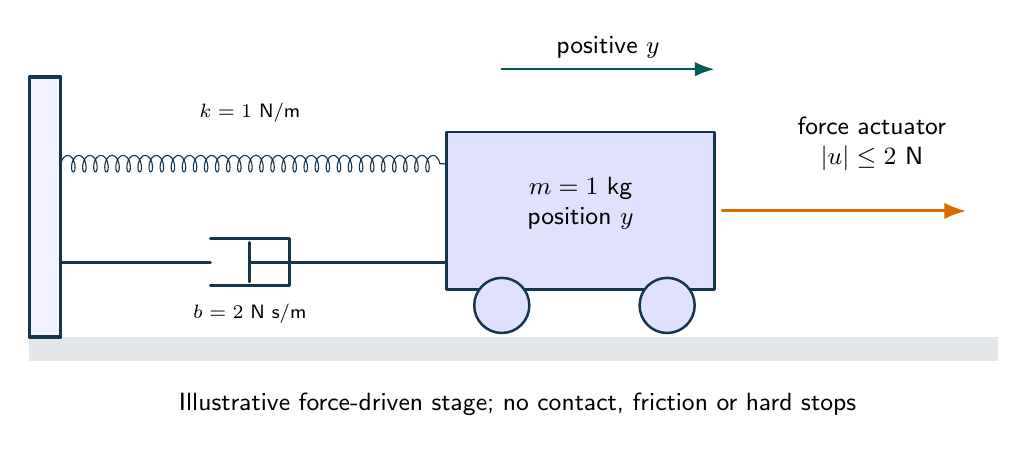
\begin{tikzpicture}[
font=\sffamily\small,>=Latex,line cap=round,line join=round,
wall/.style={draw=ink,line width=1.2pt,fill=blue!5},
water/.style={fill=cyan!25,draw=none},
metal/.style={draw=ink,fill=blue!12,line width=.9pt},
flow/.style={->,draw=blue!65!black,line width=1.2pt},
heat/.style={->,draw=orange!85!black,line width=1.1pt},
measure/.style={->,draw=teal!70!black,line width=.9pt},
dim/.style={<->,draw=ink!65,line width=.6pt},
spring/.style={draw=ink,decorate,decoration={coil,aspect=.5,segment length=4pt,amplitude=3pt}},
wire/.style={draw=ink,line width=1pt},
lab/.style={align=center,font=\sffamily\small},
smalllab/.style={align=center,font=\sffamily\scriptsize}]

\fill[ink!12](.7,.4)rectangle(13,.7);
\draw[wall](.7,.7)rectangle(1.1,4);
\draw[metal](6,1.3)rectangle(9.4,3.3);
\node[lab]at(7.7,2.4){$m=1$ kg\\position $y$};
\draw[spring](1.1,2.9)--(6,2.9);
\node[smalllab]at(3.5,3.55){$k=1$ N/m};
\draw[wire](1.1,1.65)--(3,1.65)(3,1.35)--(4,1.35)--(4,1.95)--(3,1.95);
\draw[wire](6,1.65)--(3.5,1.65)(3.5,1.4)--(3.5,1.9);
\node[smalllab]at(3.5,1){$b=2$ N s/m};
\draw[metal](6.7,1.1)circle(.35)(8.8,1.1)circle(.35);
\draw[heat](9.5,2.3)--(12.6,2.3);
\node[lab]at(11.4,3.15){force actuator\\$|u|\leq2$ N};
\draw[measure](6.7,4.1)--(9.4,4.1)node[midway,above]{positive $y$};
\node[lab]at(6.9,-.15){Illustrative force-driven stage; no contact, friction or hard stops};
\end{tikzpicture}
}\par{\small A mass, spring, damper and bounded force actuator physically realize the normalized second-order plant. Force saturation is included; contact, dry friction and travel stops are not.}\end{center}
\section{Ideal pole matching}
For an ideal PID $K_p+K_i/s+K_ds$, the closed-loop characteristic polynomial is $s^3+(2+K_d)s^2+(1+K_p)s+K_i$. Matching $(s+2)(s+3)(s+4)=s^3+9s^2+26s+24$ gives
\[K_p=25,\qquad K_i=24,\qquad K_d=7.\]
These desired poles describe an ideal linear controller, not the filtered saturated implementation.
\section{Realizable controller states}
Let $z$ be a low-pass filtered position, $\tau_f\dot z=x-z$, and let $I$ denote the integral contribution in actuator units. Define
\[e=r-x,\quad u_* = K_pe+I-K_d(x-z)/\tau_f,\quad u=\operatorname{clip}(u_*,-2,2).\]
Derivative action is applied to the measurement, avoiding the ideal derivative impulse from a reference step. The unsaturated characteristic polynomial becomes
\[\tau_fs^4+(1+2\tau_f)s^3+[2+\tau_f(1+K_p)+K_d]s^2+[1+K_p+K_i\tau_f]s+K_i.\]
Its roots must be checked separately.
\section{Windup and back-calculation}
Ordinary integration uses $\dot I=K_ie$. Back-calculation uses $\dot I=K_ie+8(u-u_*)$. The second term reduces the mismatch between requested and realizable actuator effort. It vanishes when unsaturated.
The initial command 3 is infeasible because the plant's static gain is one and the actuator limit is 2. The experiment intentionally accumulates windup, then commands a feasible target. Integrate the two time intervals separately so the reference discontinuity is not smoothed by the solver.
\section{Assessment}
Compare the integral state, output, actuator and integral absolute error after the command reduction. Back-calculation improves this particular recovery; its gain is not a universal optimum and noisy measurements or other saturation limits can change the result.
\section{What to learn from the experiment}
An infeasible command cannot be repaired by controller gain. Anti-windup improves recovery after saturation rather than increasing physical actuator capacity.
\section{System sketch}
\begin{center}\resizebox{\ifdim\width>.98\linewidth.98\linewidth\else\width\fi}{!}{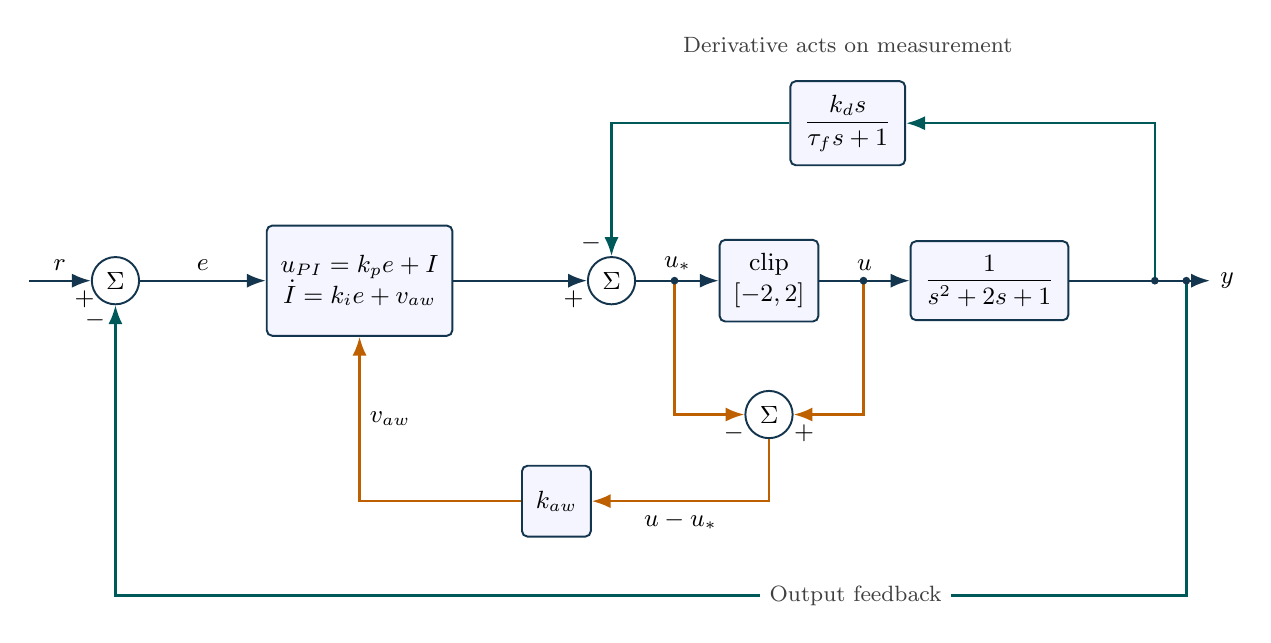
\begin{tikzpicture}[x=1cm,y=1cm,>=Latex,font=\small,
block/.style={draw=ink,fill=blue!4,rounded corners=2pt,minimum height=9mm,align=center,line width=.7pt,inner sep=5pt},
sum/.style={circle,draw=ink,fill=white,minimum size=6mm,inner sep=0pt,line width=.7pt},
sig/.style={->,draw=ink,line width=.85pt},
fb/.style={->,draw=teal!70!black,line width=.85pt},
dist/.style={->,draw=orange!75!black,line width=.85pt},
tap/.style={circle,fill=ink,inner sep=1.4pt},
note/.style={font=\footnotesize,align=center,text=black!75}]

\node[sum](e)at(.9,0){$\Sigma$};
\node[block,minimum height=14mm](pi)at(4,0){$u_{PI}=k_pe+I$\\$\dot I=k_ie+v_{aw}$};
\node[sum](tot)at(7.2,0){$\Sigma$};
\node[block](sat)at(9.2,0){$\operatorname{clip}$\\$[-2,2]$};
\node[block](plant)at(12,0){$\dfrac{1}{s^2+2s+1}$};
\draw[sig](-.2,0)--node[above]{$r$}node[pos=.9,below]{$+$}(e);
\draw[sig](e)--node[above]{$e$}(pi);
\draw[sig](pi)--node[pos=.9,below]{$+$}(tot);
\draw[sig](tot)--node[above]{$u_*$}(sat);
\draw[sig](sat)--node[above]{$u$}(plant);
\draw[sig](plant)--(14.8,0)node[right]{$y$};
\node[block](df)at(10.2,2){$\dfrac{k_ds}{\tau_fs+1}$};
\draw[fb](14.1,0)--(14.1,2)--(df);
\draw[fb](df)--(7.2,2)--node[pos=.9,left]{$-$}(tot);
\fill[ink](14.1,0)circle(1.4pt);
\node[note]at(10.2,3){Derivative acts on measurement};
\node[sum](aw)at(9.2,-1.7){$\Sigma$};
\draw[dist](10.4,0)--(10.4,-1.7)--node[pos=.85,below]{$+$}(aw);
\draw[dist](8,0)--(8,-1.7)--node[pos=.85,below]{$-$}(aw);
\fill[ink](10.4,0)circle(1.4pt);\fill[ink](8,0)circle(1.4pt);
\node[block](kaw)at(6.5,-2.8){$k_{aw}$};
\draw[dist](aw)--(9.2,-2.8)--node[below]{$u-u_*$}(kaw);
\draw[dist](kaw)--(4,-2.8)--node[right]{$v_{aw}$}(pi.south);
\draw[fb](14.5,0)--(14.5,-4)--(.9,-4)--node[pos=.95,left]{$-$}(e);
\fill[ink](14.5,0)circle(1.4pt);
\node[note,fill=white]at(10.3,-4){Output feedback};

\end{tikzpicture}
}
\par\small\refstepcounter{figure}\label{fig:system}\textbf{Figure \thefigure.} Filtered derivative acts on measurement. Back-calculation sends the actual-minus-requested actuator effort into the integral-state equation.\end{center}
\section{Executed computational evidence}
\VerbatimInput[fontsize=\small,breaklines=true]{results.txt}
\begin{center}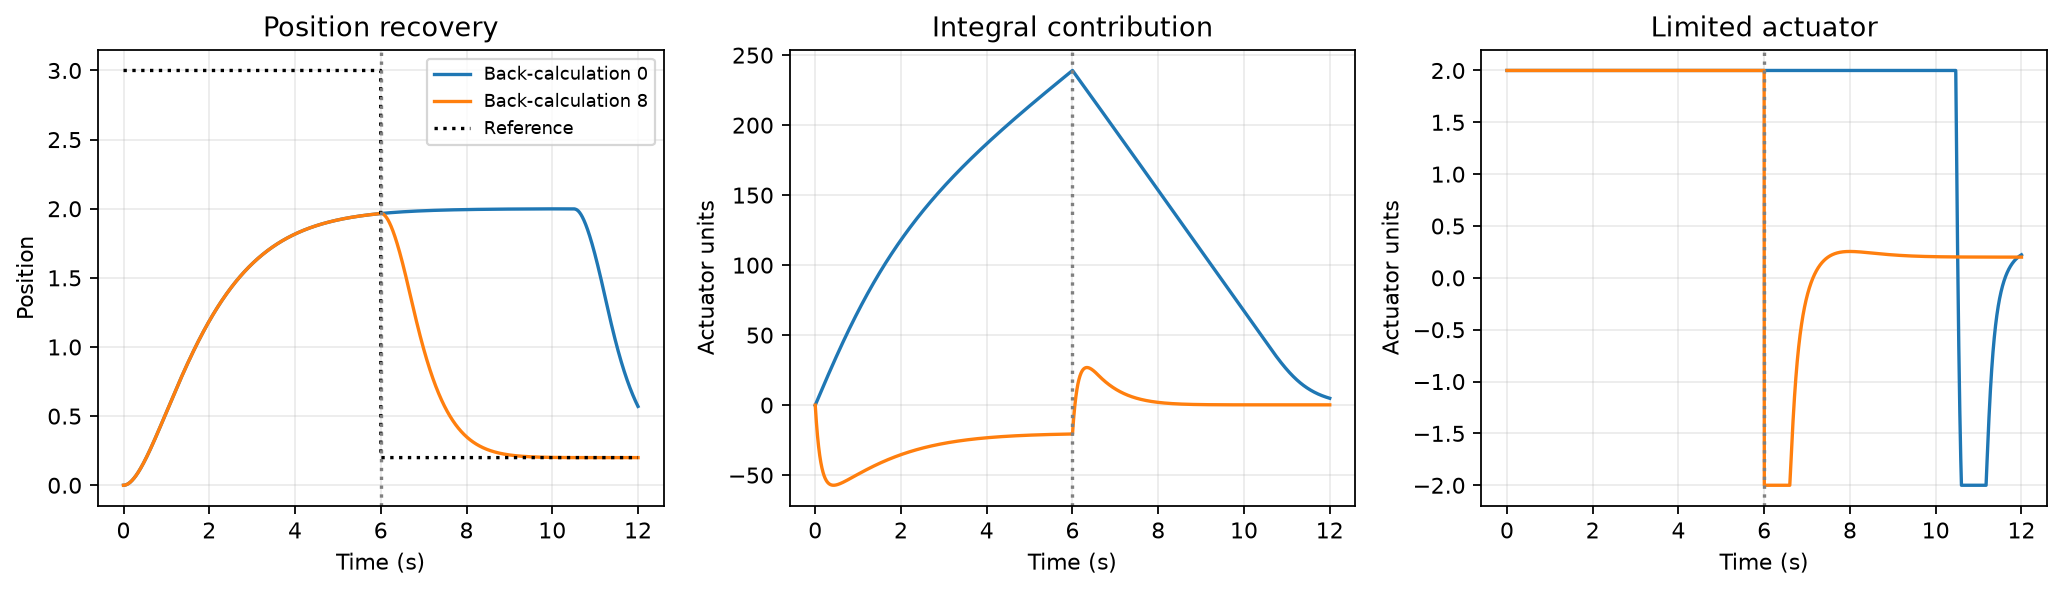
\includegraphics[width=\linewidth,height=.46\textheight,keepaspectratio]{response.png}\end{center}
\section{Method references}
The equations use standard balance laws and feedback-control methods. Further explanation: \url{https://apmonitor.com/pdc/} and \url{https://fbsbook.org/}. Implementation documentation: \url{https://python-control.readthedocs.io/en/0.10.2/}. See the repository reference catalog for individual topics and videos.
\end{document}
